\chapter{Life After Selling Your Company For \$1 Billion}

This chapter begins with a street-level question about income and opens, almost at once, into a more serious inquiry about scale, purpose, and the management of constraint. Glenn Boyd does not give us a formal theory of wealth. What he gives us is a sequence of working rules: how skill substitutes for capital, how travel changes one's estimate of the market, how attention must be budgeted in remote work, why privacy pressure gives Web3 its limited seriousness, why cybersecurity demand is structural, and why recessions must be read not only as pain but also as repricing. The mathematics here is schematic rather than formal, but it is real enough. It appears in timescales, capital thresholds, conserved attention, and causal chains.

\begin{remark}
No validated mathematical screenshots survived for this lecture, so every displayed equation and diagram below is an editorial compression of transcript-backed reasoning rather than a transcription of visible board work.
\end{remark}

\section{A Street Encounter, an Exit, and the Return to Work}

The interview is framed as an anomaly. What begins as a downtown Austin income question suddenly lands on a very different life: a founder who says, in compressed form, that he built a company, sold it when he was thirty-three, retired, and later went back to work. The number arrives early because it must; it explains why the hosts follow him for the rest of the day. But the chapter is not really about the number alone.

Glenn says that the company he founded in the original dot-com world went public in 1999 and was among the early profitable dot-com companies. Later, in a merger with another public company, it sold for roughly \$1.03 billion for the whole company. That is the hardest numerical fact in the lecture, and it is worth keeping explicit:

\begin{equation}
V_{\mathrm{sale}} \approx 1.03\times 10^{9}\ \mathrm{USD}.
\end{equation}

The next move is the important one. He retires, buys a yacht, travels around the world, spends time with his children, and then begins to get bored. The lecture thereby announces its governing paradox: the exit solves one class of problem and leaves another untouched.

\paragraph{Claim.} Capital enlarges the feasible set, but it does not abolish the need for meaningful work.

\paragraph{Mechanism.} Once immediate scarcity relaxes, other constraints become visible: boredom, purpose, the allocation of time, and the question of whether one still wants to build.

We should feel the interview pivot at this point. It does not linger over wealth display. It turns backward and asks what kind of life could have produced this founder before the exit ever happened.

\section{Scarcity, Skill, and the Decision to Found}

The next section is biographical, but not merely biographical. It explains the origin of the founder's risk tolerance and technical self-reliance. Glenn describes a poor beginning in Texas, roofing houses with his father, later washing dishes to help his mother pay rent, and then moving to Southern California as a teenager. There, somewhere between busboy work and adolescent curiosity, he begins to teach himself software.

The lecture's rhythm is causal. Programming is not introduced as a hobby insulated from money; it is introduced in the middle of economic pressure. He starts around 1980, finds that he is good at it, gets contracting work, and by sixteen is already working full time. That sequence matters.

One compact way to state the conversion is
\begin{equation}
\text{technical skill} \Longrightarrow \text{contract income} \Longrightarrow \text{time and confidence to found.}
\end{equation}

This is not a formal economic identity, but it captures the mechanism in the transcript. Before outside capital arrives, technical competence itself can function as capital. It generates cash flow; cash flow creates room for further risk; risk eventually becomes founding.

Glenn then sketches a familiar but important progression: early companies in youth, several years working for another company in his early twenties, and finally a threshold judgment. If he is going to go for it, he must do it now. The founding decision is therefore presented not as abstract inspiration but as a timing decision under uncertainty.

That tone matters. The lecture does not romanticize the moment. It places it after labor-market proof, after self-teaching, and after several attempts to enter the game from below.

\section{Travel and the Enlargement of the Market}

The interviewer next asks about travel. This could have become a decorative interlude, but Glenn treats it as a lesson in commercial scale. Travel matters because it changes the size of the world in one's head, and that, in turn, changes the estimate of what a market can be.

\paragraph{Claim.} Travel enlarges market imagination.

\paragraph{Mechanism.} Foreign sales offices, distributorships, and repeated exposure to major cities make it harder to confuse the local market with the whole field.

The examples do a great deal of work: Hong Kong, Shanghai, New York, Paris. The point is not simply that these places are large or beautiful. The point is that after moving among them, it becomes much harder to think provincially. One no longer reasons from one national or regional demand curve; one begins to think in terms of world scale.

Later in the same discussion, the travel question narrows. The interviewer asks for places to recommend, and Glenn answers by objective. China appears as the overwhelming lesson in urban scale and economic scope; Italy appears as a personal favorite; Norway appears under the sign of beauty and the memory of a dear friend. That split is worth preserving. Even in casual recommendation, he distinguishes between travel for business perspective and travel for life.

We should therefore write this section with some care. The lecture is not saying that travel is merely luxurious. It is saying that travel corrects a founder's estimate of what is possible.

\section{Routine, Momentum, and the Management of Attention}

After scale, the interview narrows sharply into daily rhythm. Glenn is asked about his morning routine, and the answer is almost aggressively ordinary: make coffee, get on the computer, respond to email, write to-do lists, keep several threads moving at once. Later, when the workday question returns, he adds architecting, design, sketches, workflows, hikes, and shifting to a shared workspace on another floor.

The lecture's point is not that routine is glamorous; it is that scale is built on routine. Lists matter because there are usually several live tasks. Remote work matters because it changes the texture of concentration. Health matters because long isolated stretches of work can lower the quality of later thinking.

We can summarize one of Glenn's strongest practical claims by the schematic relation
\begin{equation}
H_{\mathrm{continuous\ work}}\uparrow \Longrightarrow C_{\mathrm{creativity}}\downarrow.
\end{equation}

Here \(H_{\mathrm{continuous\ work}}\) stands for repeated long stretches of uninterrupted work, and \(C_{\mathrm{creativity}}\) for effective creative output. The interview gives no measured function; it gives only the direction. Too many days of eight-, ten-, or twelve-hour isolation eventually leave one staring at the screen rather than producing.

\paragraph{Claim.} The workday is not maximized by duration alone.

\paragraph{Mechanism.} In a remote environment, uninterrupted concentration can overshoot; breaks, movement, and changes of workspace preserve rather than destroy output.

There is also a smaller but revealing heuristic in the task-prioritization exchange. The transcript becomes garbled at exactly the point where Glenn describes the fine structure of sequencing, so we should be cautious. But one usable line survives: it can be helpful to begin with something easy or appealing, simply to break the ice and get motion started. What follows after that appears to be a kind of bouncing or stitching among tasks, some related and some not, rather than a rigid linear queue.

This is the right place to notice the deeper tone of the interview. Enormous outcomes are repeatedly traced back to mundane operating behavior: coffee, email, lists, sketching, movement, and the management of mental energy.

\section{Web3, Privacy, and the Search for a Real Use}

Only after the interview has established biography, scale, and routine does it widen again into contemporary technology. Glenn is asked about cryptocurrency, Web3, and recent blockchain developments. He does not answer by enumerating protocols. He mentions proof of stake and proof of work briefly, and notes the environmental improvement associated with the former. But he quickly shifts from implementation detail to the more basic question: what problem makes any of this matter?

\subsection{Question \& Answer}

\paragraph{Question.} What is Web3 actually solving?

\paragraph{Answer.} Glenn's answer is social and commercial rather than purely technical. People are increasingly frustrated with digital systems whose business model is advertising and whose working material is personal information. Younger generations, in his description, are more alert to privacy and less willing to have all social interaction monetized by centralized platforms. In that setting, Web3 becomes interesting insofar as it offers a mechanism for distributed applications and distributed social interaction that does not depend in the same way on selling the user back to advertisers.

One clean way to record that is
\begin{equation}
\text{privacy concern} + \text{resistance to ad-monetization}
\Longrightarrow D_{\mathrm{decentralized\ apps}}\uparrow.
\end{equation}

A second ingredient then enters. Glenn broadens the scope from privacy to the decentralization of work itself. If white-collar labor is increasingly remote and geographically distributed, then the desire for easier, faster, and less centralized digital transactions grows along with it.

\begin{figure}[h]
\centering
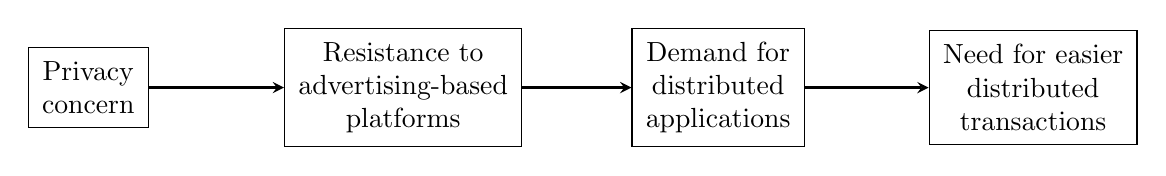
\begin{tikzpicture}[>=stealth]
\node[draw, rectangle, align=center, inner sep=5pt] (p) at (0,0) {Privacy\\concern};
\node[draw, rectangle, align=center, inner sep=5pt] (a) at (4,0) {Resistance to\\advertising-based\\platforms};
\node[draw, rectangle, align=center, inner sep=5pt] (d) at (8,0) {Demand for\\distributed\\applications};
\node[draw, rectangle, align=center, inner sep=5pt] (t) at (12,0) {Need for easier\\distributed\\transactions};
\draw[->, thick] (p) -- (a);
\draw[->, thick] (a) -- (d);
\draw[->, thick] (d) -- (t);
\end{tikzpicture}
\caption{An editorial schematic of the Web3 motivation as it is given in the interview.}
\end{figure}

We should be disciplined here. The lecture does not derive a blockchain theorem. It does not present token economics or consensus mathematics. What it does present is a credible motivating chain: privacy pressure, dissatisfaction with ad-based centralization, distributed interaction, and the need for payment rails that match a more distributed world.

\section{Cybersecurity and the Growth of the Attack Surface}

The interview then makes one of its strongest pivots. Once we begin talking about distributed systems, remote work, and digitized infrastructure, the next question is no longer aspiration but vulnerability. The interviewer names recent hacks and asks how important cybersecurity will become over the next ten or twenty years. Glenn answers immediately: massive.

\begin{definition}
The \emph{attack surface} is the effective digital exposure created by remote access, cloud dependence, interconnection, and insecure design.
\end{definition}

The causal structure is simple and strong:
\begin{equation}
\text{cloud interconnection} + \text{weak security design}
\Longrightarrow A_{\mathrm{attack\ surface}}\uparrow
\Longrightarrow D_{\mathrm{security\ labor}}\uparrow.
\end{equation}

This is not a statement about cybercrime as a passing trend. It is a statement about the architecture of the world we have built. Security, Glenn says, is only now starting to be treated as a design-stage concern rather than an afterthought. His analogy is memorable precisely because it is so plain: we built these structures as though they were buildings without proper locks and doors, and then seemed surprised when people walked in.

The lecture then grounds the abstraction historically. Glenn says he started in information security early enough to train agencies such as the FBI, the CIA, and the IRS. Those institutions used to build cases from file cabinets. Then they entered rooms with no cabinets at all, only computers. Early forensic work therefore meant something concrete: showing agents how to recover deleted documents and extract information from machines they did not yet know how to read.

\paragraph{Claim.} Security demand grows because the medium of evidence, work, and failure becomes digital.

\paragraph{Mechanism.} Once information migrates from paper into computers, then into networks, then into cloud-based systems, compromise becomes easier, broader, and more consequential. Security expertise therefore becomes structurally necessary.

\begin{figure}[h]
\centering

\begin{tikzpicture}[>=stealth]
\node[draw, rectangle, align=center, inner sep=5pt] (f) at (0,0) {File cabinets\\and paper records};
\node[draw, rectangle, align=center, inner sep=5pt] (c) at (4,0) {Computers as\\evidence stores};
\node[draw, rectangle, align=center, inner sep=5pt] (r) at (8,0) {Forensic recovery\\of digital data};
\node[draw, rectangle, align=center, inner sep=5pt] (n) at (12,0) {Cloud and network\\interconnection};
\node[draw, rectangle, align=center, inner sep=5pt] (s) at (16,0) {Security by design\\as permanent demand};
\draw[->, thick] (f) -- (c);
\draw[->, thick] (c) -- (r);
\draw[->, thick] (r) -- (n);
\draw[->, thick] (n) -- (s);
\end{tikzpicture}
\caption{An editorial schematic of the interview's security narrative: digitization changes evidence, exposure, and labor demand.}
\end{figure}

We should also notice how this section feeds forward. Later, when the interviewer asks what field a young person should consider for a durable career, Glenn returns to information security. The chapter's technology discussion is therefore not merely commentary on the state of the industry; it is also labor-market advice.

\section{Founder Filters, Family Time, and Capital in Recession}

After the large field-level claims about Web3 and security, the interview narrows once more into the personal scale of founding. Glenn is asked about ideas for companies that did not happen. His answer is that ideas are the easy part and doing is the hard part. He often carries ideas through an initial filter: what would the business actually be, what is its viability, what is the competition, and, more deeply, if it succeeded, would he want to spend years inside it?

That last question is the decisive one, because the lecture keeps refusing short-term glamour. A company is not simply an exit option. It is a multi-year environment in which one must live.

\begin{equation}
T_{\mathrm{build}} \gtrsim 3\text{--}5\ \mathrm{years}.
\end{equation}

This timescale is one of the chapter's clearest quantitative anchors. Even very successful companies usually require at least that long. So the founder's selection problem is not merely ``Is this clever?'' It is also ``Can I bear to inhabit this problem for years?''

A useful two-stage filter is therefore:
\begin{enumerate}
\item Is the business viable enough to merit real investigation?
\item If it works, do we want to spend \(3\text{--}5\) years living inside it?
\end{enumerate}

The interview then sharpens the matter by moving from abstract ideas to family time. Asked about the biggest challenge in the first company, Glenn answers bluntly: there were not enough hours in the day. Young children, employees lined up outside the office, product questions, administrative needs, and home responsibilities all press on the same finite resource.

We may write the constraint schematically as
\begin{equation}
H_{\mathrm{family}} + H_{\mathrm{team}} + H_{\mathrm{product}} + H_{\mathrm{admin}}
= H_{\mathrm{available}}.
\end{equation}

Again, this is not claimed as a formula Glenn wrote down. It is the cleanest summary of the anecdote: the day is finite; the claims on it are not.

Later in the same general movement, the interview asks what someone should do with about \$100{,}000 and then, more broadly, what financial advice Glenn has for younger people in a weak economy.

\subsection{Question \& Answer}

\paragraph{Question.} What should one do with limited capital in a weak economy?

\paragraph{Answer.} Glenn's answer is intentionally conservative. With only about \$100{,}000, one should not behave as if one has the balance sheet required for immediate capital-intensive high-tech buildout. One should either begin with a service business that produces income or, if one has the technical skill, invest labor directly and build the first version oneself.

\begin{equation}
C_{0} \approx 10^{5}\ \mathrm{USD}
\Longrightarrow \text{service revenue first or founder-built product.}
\end{equation}

That advice connects naturally to his remarks on recession. Downturns are painful, but they are also repricing events. Labor becomes cheaper. Certain services become cheaper. Even remodeling gets cheaper, which is why, Glenn says, he has sometimes waited for a recession before doing work on a house. The same logic applies to hiring and company formation.

We can turn that spoken logic into a small proposition.

\begin{proposition}
For fixed deployable capital \(K\), if recession lowers the unit labor cost from \(c_{1}\) to \(c_{2}\) with \(c_{2}<c_{1}\), then the amount of labor purchasable with the same capital strictly increases.
\end{proposition}

\begin{proof}
If purchasable labor is
\begin{equation}
Q_{\mathrm{labor}}=\frac{K}{c_{\mathrm{labor}}},
\end{equation}
then before the repricing we have \(Q_{\mathrm{labor}}=K/c_{1}\), and after it we have \(Q'_{\mathrm{labor}}=K/c_{2}\). Hence
\begin{align}
Q'_{\mathrm{labor}}-Q_{\mathrm{labor}}
&= \frac{K}{c_{2}}-\frac{K}{c_{1}} \\
&= K\left(\frac{1}{c_{2}}-\frac{1}{c_{1}}\right) > 0,
\end{align}
because \(c_{2}<c_{1}\) implies \(1/c_{2}>1/c_{1}\).
\end{proof}

That is the mathematical core of Glenn's recession advice. If the founder has savings and patience, the same capital can purchase more real input during a downturn. This does not mean recession is good in every sense; it means recession is not only bad in the sense people commonly imagine. The lecture insists that downturns are temporary, and that one mistake people make is to read temporary difficulty as permanence.

We should keep a further caution here. Glenn's explanation of inflation includes pandemic disruption, supply-chain effects, and corporate greed. Those are his explanatory claims, not settled macroeconomic laws. The durable practical rule is narrower: maintain liquidity, do not panic, and remember that repricing changes what capital can buy.

The last advisory move is about informational discipline. Asked how one knows when it is a good time to buy into a certain industry, Glenn warns against the shotgun method: hearing about something only after everyone else is already excited and then running in circles between sectors. His alternative is to stay with what one knows, or to learn one field deeply enough that judgment becomes first-hand.

\begin{equation}
\text{domain depth}\uparrow \Longrightarrow \text{decision quality}\uparrow.
\end{equation}

This is not a theorem. It is an investing and career heuristic. But it is one of the lecture's cleanest closing rules.

\section{Summary}

The interview begins with a spectacular number and ends with a more durable set of constraints. We start with a billion-dollar exit, but the lasting payload lies elsewhere: scarcity converted into skill, travel converted into market scale, routine converted into output, privacy pressure converted into demand for distributed systems, interconnection converted into attack surface, and fixed capital converted into opportunity or failure depending on timing and depth of knowledge.

The lecture's deepest lesson is therefore not that one large win solves life. It is that after the win, and even before it, one is still governed by time, attention, skill, market size, and the price of inputs. In that sense these notes are not a celebration of wealth at all. They are a study of how judgment moves inside changing constraints.